Pour créer le corpus, nous combinerons les 3 échanges de textos en un seul texte séparé par des espaces entre chaque texto. Ainsi, cet échange :
\begin{enumerate}
\item Don't worry  I'm girl
\item hmm how do I know if you are
\item What's ur name?
\end{enumerate}
Devient :\textbf{Don't worry  I'm girl hmm how do I know if you are  What's ur name?} . Ce qui forme le premier texte de notre corpus. Le même processus est appliqué à tous les autres textes.

Pour transformer les mots de notre corpus sous une forme numérique, nous testerons 3 modèles différents : le compte de mots, la présence de mots (0 ou 1) et la valeur TF-IDF (term frequency-inverse document frequency). Pour chacun d'entre eux, nous retirerons les mots outils (\emph{stop words}. Les seuls paramètres qui seront modifiés sont : le nombre de n gram utilisés et la fréquence minimale conservée pour chaque n gram.

Il est noté qu'on conservera toutes les classes de mots et aucun stemming ne sera appliqué étant donné la nature des textes avec lesquels on travaille:

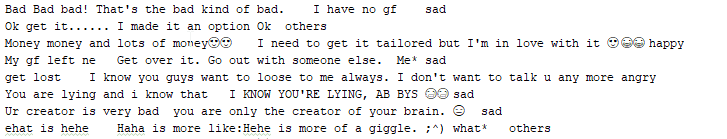
\includegraphics[width=\linewidth,height=5cm]{images/exemples_text}

On peut voir que certains mots sont inventés, d'autres mal écrits et certains sont des abréviations. Par conséquent, le stemming ou la conservation de classe ouverte seulement ne serait pas une bonne idée puisque beaucoup d'information serait perdue.

En conclusion, la matrice de données utilisée pour nos modèles de classification sera composée de données d'un des 3 objets de compte décrits dans cette sous-section avec ou sans les attributs supplémentaires décrits dans la section \emph{Analyse préliminaire des données} (si \verb|bool_ajouter_autres_features=True|).